\documentclass[a0paper,fleqn]{betterposter}

%%%% Configuration (omitting most of the unused settings for brevity)



\renewcommand{\maincolumnbackgroundcolor}{methods}
\usepackage{caption}
\captionsetup{
	font=LARGE,       % set the font size to 'large' for both label and text
	labelfont=LARGE   % set the font size to 'large' for the label
}
\usepackage[square,numbers]{natbib}
\renewcommand{\bibfont}{\LARGE}
\begin{document}    
	\betterposter{
		%%%%%%%% SINGLE LEFT COLUMN (MERGED)
		
		\title{Application of the LISFLOOD-FP \\Hydrodynamic Model for Impact-Based Forecasting over the Eastern Africa \\Region}
		 \vspace{1em}%
		\section{
			\begin{minipage}[c]{0.07\textwidth}
				\includegraphics[width=\linewidth]{img/logo2.png}
			\end{minipage}%
		    \hspace{0.5em}%
			\begin{minipage}[c]{0.07\textwidth}
				\includegraphics[width=\linewidth]{img/logo1.png}
			\end{minipage}%
		    \hspace{1em}%
			\begin{minipage}[c]{0.9\textwidth}
				Jully Ouma$^{1,2}$, \underline{Nishadh Kalladath$^{1}$}, Khalid Hassaballah$^{1}$, Viola Otieno$^{1}$, Jason Kinyua$^{1}$, 
				\vspace{0.4em}%
				\\ Igbal Salah$^{1}$, Mohammed Hassan$^{1}$, Ahmed Amdihun$^{1}$ \& Guleid Artan$^{1}$
				\vspace{0.8em}%
				\\${^1}$ IGAD Climate Prediction and Applications Centre- ICPAC, Nairobi, Kenya
				\\${^2}$ United Nation Office for Disaster Risk Reduction, Africa Office, Kenya
			\end{minipage}
		}
	    \vspace{1em}%
		\hrule
		
		\section{Introduction}
		\begin{itemize}
			\item Impact-based forecasting (IBF) aims to support risk-oriented decisions in disaster risk management by promoting anticipatory actions that minimize damage and loss of life from natural hazards
			\item The floodplain inundation data is required for impact functions that demonstrate the relationship between inundation depth and displacement probability, as well as economic damage to buildings, roads, and commercial/agriculture land use categories
			\item Widely available hydrological models typically use streamflow rate forecasts in conjunction with historical flood hazard maps to derive inundation maps, but this method lacks specificity in capturing rainfall-induced catchment and flash flooding processes, especially in riverine and urban areas
			\item In this study, we tested the hydrodynamic model LISFLOOD-FP \cite{sharifian2023lisflood} for impact-based forecasting and assessed the operational IBF suitability of the parsimonious, simplified model RIM2D \cite{apel2022brief}
			
		\end{itemize}
		
		\section{Methods}
		\\ Method used for compare the LISFLOOD-FP and RIM2D operational purpose in Cloud computer.
		\begin{center}
		%\begin{figure}[h!]	
			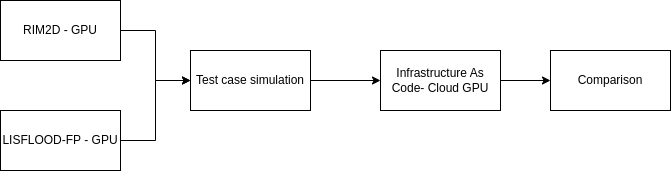
\includegraphics[width=\textwidth]{img/rim2d.png}
			\captionof{figure}{\LARGE{GPU version of the models are used in similar GPU Cloud Computing setup}}
		%\end{figure}
		\end{center}
		
	    \section{Results}
		\begin{itemize}
			\item Initial simulations indicate RIM2D is more efficient for operational IBF due to its parsimonious hydrological modeling approach, making it apt for IBF risk measures
			\item The validity of RIM2D's hydrodynamic modeling in East Africa is underway; the provided GitHub repository details the Python programs and cloud setup for the model
	
			%\item Study is ongoing to extend the application
		\end{itemize}
		%% Institution logo
		%\includegraphics[width=\textwidth]{img/logo}\\
		\section{Reference}
		%\begin{enumerate}
		%\item 
		%\item OpenAI. "GPT-4 Technical Report." arXiv e-prints, 2023, arXiv:2303.08774.
		%\item Ankan, Ankur, and Abinash Panda. 2015. [4]. 
		%\item Ankan, Ankur, and Abinash Panda. 2015. [4] \LARGE{"pgmpy: Probabilistic graphical models using python." Proceedings of the 14th python in science conference (scipy 2015). Vol. 10. Citeseer, 2015.}
		%\item \url{github.com/nishadhka/bn-ibf/code/01-simple-bn-flood.ipynb }
		\renewcommand{\bibsection}{}                                                                                                               
		\bibliographystyle{unsrtnat} % or another suitable style like abbrvnat, unsrtnat, etc.
		\bibliography{references} % if your file is named references.bib
		
		
	    %\end{enumerate}
		
		%\author{Mike Morrison}
		%\author{Rafael Bailo}
		%\institution{Optional Institution Under Name}
	}	
	{
		%%%%%%%% MAIN COLUMN
		\maincolumn{
			%%%% Main space
						
		\textbf{RIM2D}, a streamlined, \textbf{parsimonious} version of \textbf{LISFLOOD-FP} model, might be the ideal choice for \textbf{impact-based forecasting}. After all, why putting on a \textbf{space suit} to water the \textbf{garden}?
			
		}{
			%%%% Bottom space
			\qrcode{img/qrcode-rim2d}{img/smartphoneWhite}{
				\textbf{Scan here} to proceed
				\\Github repo project
				\\icpac-igad/rim2d-ibf
				\\\textbf{For comments and questions}
				\\icpac-igad/rim2d-ibf/issues
			}
		}
		
	}
	
\end{document}
